% !TeX spellcheck = en_US
\section{Problem 4}

In this problem, we are asked to write a program that implements backpropagation algorithm for an $1 - S^1 - 1$ network with $S=\left\{2,8,12\right\}$, as shown in figure~\ref{fig:prob4_nns}.

The first layer has $logsig$ as activation function and the output layer has $ReLU$ as activation function. Also, every weight and bias is initialized to a uniformly random number in $\left(-0.5, 0.5\right)$.
All of the above are done in order to train our network to approximate the following function:
\[
g(p) = 1 + e^{p\left(\dfrac{3\pi}{8}\right)}, \qquad p \in \left[-2,2\right]
\]

This means that, during training, we have to train the network for multiple input data (\textit{specifically, for all input data}).

\begin{figure}[htbp]
	\centering
	\begin{subfigure}{0.47\textwidth}
		\centering
		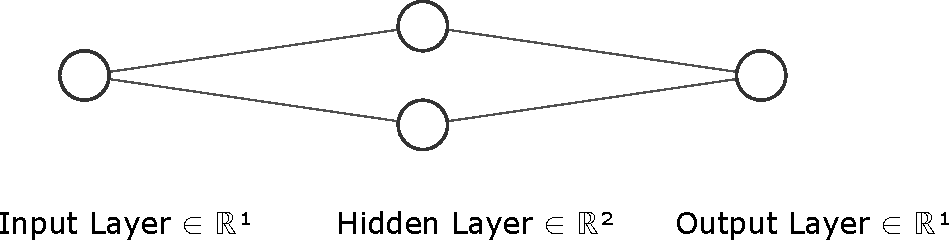
\includegraphics[width=0.9\textwidth]{../Problem 4/nn_1_2_1.pdf}
		\caption{}
	\end{subfigure}
	\begin{subfigure}{0.47\textwidth}
		\centering
		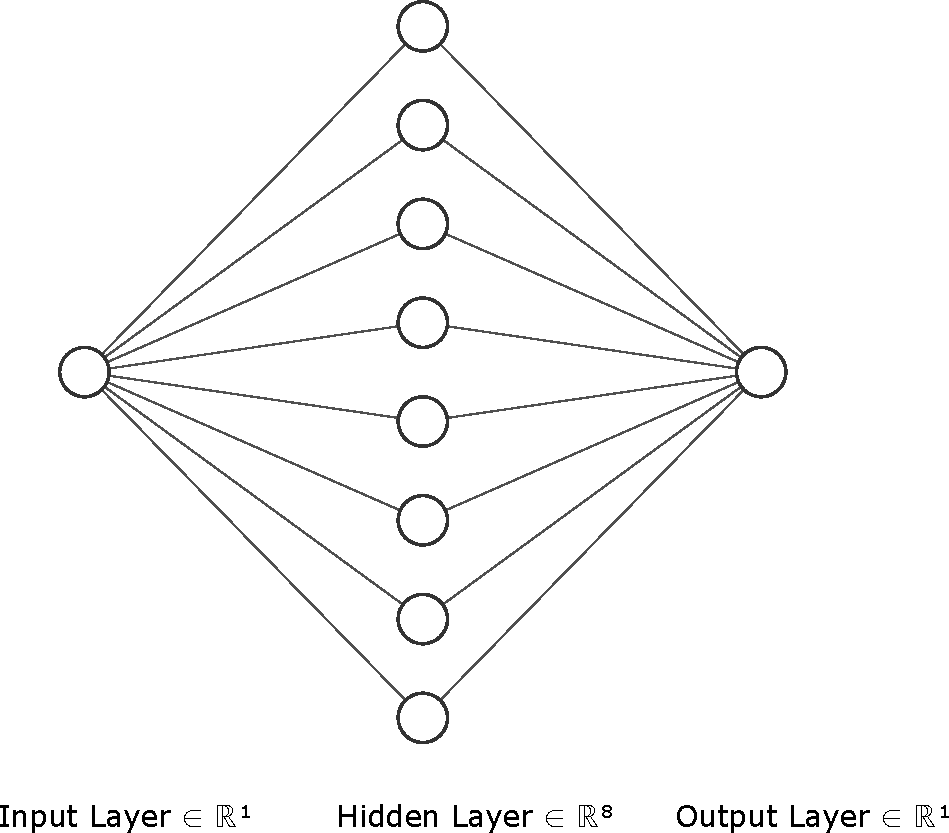
\includegraphics[width=0.9\textwidth]{../Problem 4/nn_1_8_1.pdf}
		\caption{}
	\end{subfigure}
	\begin{subfigure}{0.47\textwidth}
		\centering
		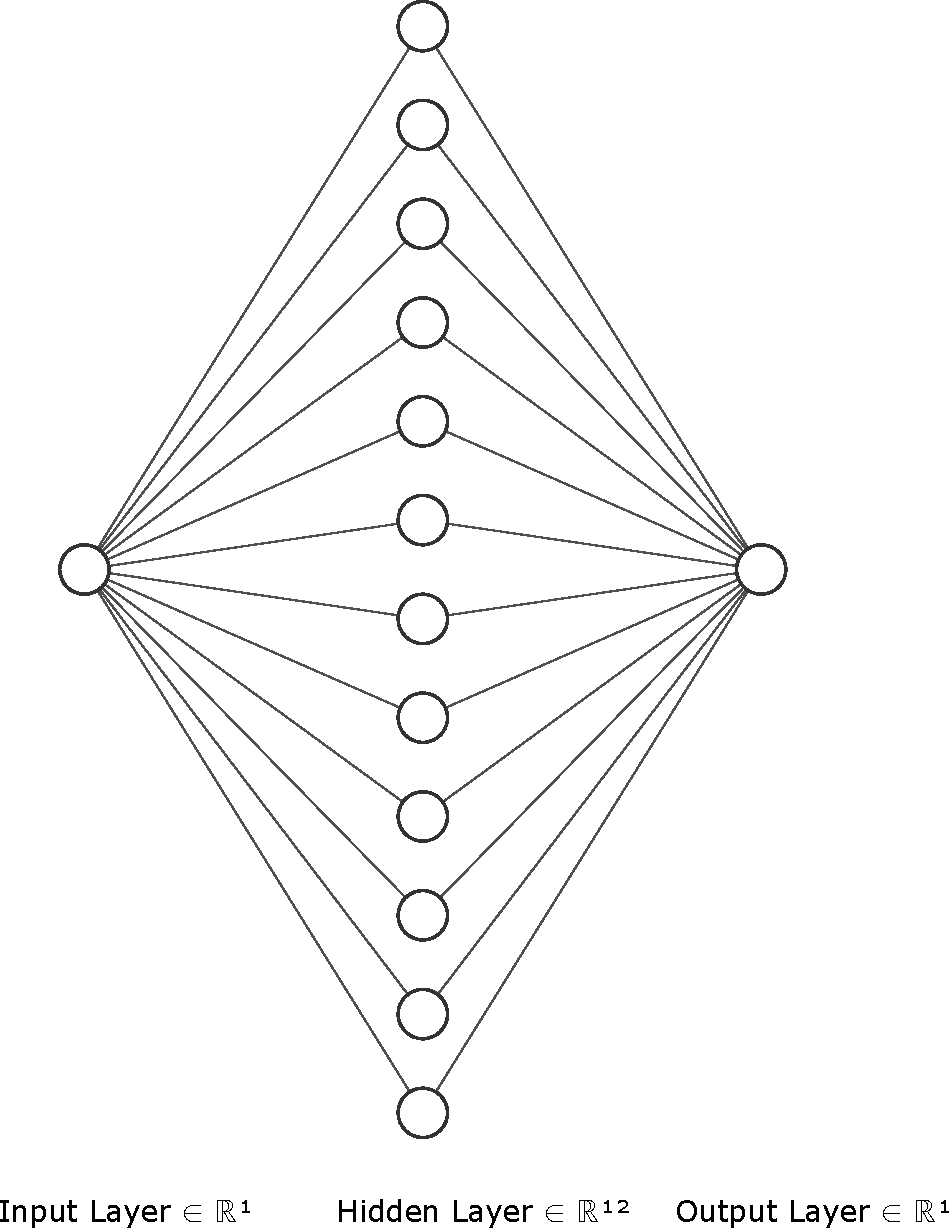
\includegraphics[width=\textwidth]{../Problem 4/nn_1_12_1.pdf}
		\caption{}
	\end{subfigure}
	\caption{All the neural networks in this problem.}
	\label{fig:prob4_nns}
\end{figure}

We chose to write this program in MATLAB, despite the majority of these problems being written in Python. This ensures that we are going to use matrix operations for initialization of all weights and biases. The code that contains all of these is inside the file "\verb*|backpropagation.m|".\\

In order to see what difference $S$ and learning rate does to our network, we defined the following learning rates $\left[0.1, 0.01, 0.001\right]$ and generated the network's output and error throughout training.
